\chapter{Goniometria}
\label{sec:GONIOMETRIA}
\minitoc
\mtcskip                                % put some skip here
\minilof                                % a minilof
\mtcskip                                % put some skip here
\minilot
\FloatBarrier
\section{Angoli}
\label{sec:gonioang}
\begin{definizione}[Angolo]
Un angolo\index{Angolo} è la parte di piano compreso fra due semirette dette lati hanno in comune l'origine chiamata vertice.
\end{definizione}

Le  semirette formano due angoli  uno convesso\index{Angolo!convesso} l'altro concavo\index{Angolo!concavo} come nella figura\nobs\vref{fig:angconconvposoneg}. 
\begin{figure} %[htbp]
	\centering
\includestandalone[width=.6\textwidth]{funzgonioTikz/angoliconcaviconvessi}
	\caption{Angoli concavi e convessi, positivi e negativi}
	\label{fig:angconconvposoneg}
\end{figure}
\begin{figure} %[htbp]
	\centering
\includestandalone[width=\textwidth]{funzgonioTikz/angolinotevoli}
	\caption{Angoli notevoli}
	\label{fig:Angolorettoposneggonio}
\end{figure}
\begin{figure}
\includestandalone[width=\textwidth]{funzgonioTikz/mappagomiometricaangolo}
	\caption{Mappa goniometria l'angolo}
	\label{fig:MappaGonometria1}
\end{figure}
\begin{definizione}[Angoli Positivi e Negativi]
	Fissato un lato, l'angolo è  positivo\index{Angolo!positivo}  se per costruirlo ruoteremo l'altra semiretta in senso antiorario.  Un angolo è negativo\index{Angolo!negativo} se ruoteremo l'altro lato in senso orario come nella figura\nobs\vref{fig:angconconvposoneg}. ...
\end{definizione}

\begin{definizione}[Angolo giro]
Un angolo è giro\index{Angolo!giro} quando le due semirette coincidono. 
\end{definizione}
\begin{definizione}[Angolo piatto]
Un angolo è  piatto\index{Angolo!retto} quando i suoi lati  coincidono con la stessa retta.
\end{definizione}
\begin{definizione}[Angolo retto]
Avremo un angolo è retto\index{Angolo!retto} quando è la metà di un angoli piatto. 
\end{definizione}
\begin{definizione}[Angolo acuto]
Un angolo è acuto\index{Angolo!acuto} se  minore di un  retto.
\end{definizione}
\begin{definizione}[Angolo ottuso]
Un angolo è ottuso\index{Angolo!ottuso} se  maggiore di un  retto.
\end{definizione}
 La figura\nobs\vref{fig:Angolorettoposneggonio} mostra  vari casi
\section{Misura dell'angolo}
\label{sec:MisuraAngoloGonio}

A ogni angolo viene associata una grandezza detta ampiezza.  Per misurare l'ampiezza dell'angolo si usa o il grado sessagesimale  o i radianti
\subsection{Angolo sessagesimale}
\begin{definizione}[Grado]
Un grado\index{Grado} è la trecentosessantesima parte in un angolo giro. Il grado si suddivide in minuti e  secondi. Il minuto è la sessantesima parte di un grado. Il secondo è la sessantesima parte di un minuto. Il secondo è suddiviso in decimi e centesimi.
\end{definizione}
 Quindi \[\ang{;1;}=\dfrac{\ang{1}}{60}\] e  \[\ang{;;1}=\dfrac{\ang{;1;}}{60}=\dfrac{\ang{1}}{3600}\]
\begin{esempio}
L'angolo  \ang{45;30;20}  ha l'ampiezza di \ang{45} gradi \ang{;30;} minuti e \ang{;;20} secondi. L'angolo \ang{30;45;23,7} secondo ha l'ampiezza di \ang{30} gradi \ang{;45;} minuti e \ang{;;23} secondi e $7$ decimi.
\end{esempio}
Un angolo giro\index{Angolo!giro} è quindi ampio \ang{360} gradi. L'angolo piatto\index{Angolo!piatto},  metà di un angolo giro, ha l'ampiezza di \ang{180} gradi. L'angolo retto\index{Angolo!retto}  metà di una angolo piatto, ha ampiezza di \ang{90} gradi.

Un angolo espresso in gradi sessagesimali può essere scritto in forma decimale. 
\begin{esempio}
 Abbiamo un angolo di ampiezza pari a \ang{44;58;48} e vogliamo scriverlo in forma decimale\index{Grado!dorma decimale} .Dato che $\ang{;1;}=\dfrac{\ang{1}}{60}$ e che $\ang{;;1}=\dfrac{\ang{;1;}}{60}=\dfrac{\ang{1}}{3600}$  avremo
\begin{align*}
	\ang{44;58;48}&=\ang{44}+\left(\dfrac{58}{60}\right)^{\circ}+\left(\dfrac{48}{3600} \right)^{\circ}\\
	&=\ang{44}+\left(\dfrac{29}{30}\right)^{\circ}+\left(\dfrac{3}{225} \right)^{\circ}\\
	&=\ang{44}+\left(\dfrac{6+435}{450} \right)^{\circ}\\
	&=\ang{44}+\left(\dfrac{441}{450} \right)^{\circ}\\
	&=\ang{44}+\num{0,98}^{\circ}\\
	&=\num{44,98}^{\circ}
\end{align*}
\end{esempio}
\begin{esempio}
Convertiamo $7,42^{\circ}$ in gradi minuti e secondi:
\begin{align*}
	7,42^{\circ}&=7^{\circ}+0,42^{\circ}\\
	&=\ang{7}+0,42\cdot \ang{1}\\
	&=\ang{7}+0,42\cdot \ang{;60;}\\
	&=\ang{7;25,2;}\\
	&=\ang{7;25;}+\ang{;0,2;}\\
	&=\ang{7;25;}+0,2\cdot\ang{;1;}\\
	&=\ang{7;25;}+0,2\cdot\ang{;;60}\\
	&=\ang{7;25;12}\\
\end{align*} 
\end{esempio}
\subsection{Radianti}
\begin{definizione}[Radiante]\index{Radiante}
Data una circonferenza di raggio $r$ e  un angolo $\alpha$ con il vertice nel centro $C$ della circonferenza, come nella figura\nobs\vref{fig:radinatidefgonio}. Se $l$ è la lunghezza dell'arco di circonferenza sotteso dall'angolo, chiamo radiante il rapporto \[\rho=\dfrac{l}{r} \]
\end{definizione}
\begin{figure}
	\centering
	\includestandalone[width=7.5cm]{funzgonioTikz/radianti}
	\caption{Radianti}
	\label{fig:radinatidefgonio}
\end{figure}
Avremo quindi che un angolo ha l'ampiezza di un radiante\index{Radiante} se l'arco di circonferenza $l$ è uguale al raggio $r$.

In un angolo giro\index{Angolo!giro} l'arco è lungo quanto la circonferenza. La sua misura in radianti è \[\rho=\dfrac{2\pi r}{r}=2\pi\]. 

Un angolo piatto, meta di un giro,  misura  \[\rho=\pi\]\index{Angolo!piatto} e  un angolo retto\index{Angolo!retto} misura \[\rho=\dfrac{\pi}{2} \] 

Per convertire  da gradi sessagesimali a radianti\index{Grado!radiante!conversione} si procede in questo modo:
\begin{align*}
\dfrac{l}{2\pi r}&=\dfrac{\alpha}{\ang{360}}\\
\dfrac{\rho}{2\pi}&=\dfrac{\alpha}{\ang{360}}\\
\rho&=\dfrac{\alpha 2\pi}{\ang{360}}\\
\rho&=\dfrac{\pi}{\ang{180}\alpha}
\intertext{segue che per passare da radianti a gradi sessagesimali avremo}
\alpha&=\dfrac{\ang{180}}{\pi}\rho
\end{align*}
Alcuni semplici esempi di conversione fra angoli e radianti
\begin{esempio}
Quanto corrisponde in gradi un radiante
\begin{align*}
\alpha&=\dfrac{\ang{180}}{\pi}\rho \\
&=\dfrac{\ang{180}}{\pi}\cdot 1\\
&\simeq\ang{57.2957}\cdot 1\\
&\simeq\ang{57.30}
\end{align*} 
\end{esempio}

\begin{esempio}
	Quanto corrisponde in radianti un grado
	\begin{align*}
	\rho&=\dfrac{\pi}{\ang{180}}\alpha \\
	&==\dfrac{\pi}{\ang{180}}\cdot 1\\
	&\simeq\ang{0.01745}\cdot 1\\
	&\simeq\ang{0.017}
	\end{align*} 
\end{esempio}

\section{Funzioni goniometriche}
\label{sec:FunzioniGoniometriche}
\begin{definizione}[Circonferenza goniometrica]
	Dato un sistema di riferimento cartesiano ortogonale, una circonferenza goniometrica\index{Circonferenza!goniometrica} è una circonferenza con centro nell'origine e raggio uguale a uno. 
\end{definizione}
\begin{figure}
	\centering
\includestandalone[width=7.5cm]{funzgonioTikz/circonferenzagoniometrica}
	\captionof{figure}{Circonferenza goniometrica}
	\label{fig:circonferenzagonimetricagonio}
\end{figure}
 La circonferenza incontra gli assi in quattro punti. $A(1,0)$, $B(0,1)$, $C(-1,0)$ e $D(-1,0)$. Costruiamo un angolo  $\alpha$  in modo che il suo vertice coincida con il centro della circonferenza. L'angolo incontra la circonferenza nei punti $A$ e $P$ come nella  figura\nobs\vref{fig:circonferenzagonimetricagonio}. 
\subsection{Coseno}
\label{sec:cosenogonio}
\begin{figure}
	\begin{subfigure}[b]{.5\linewidth}
		\centering
		\includestandalone[width=5cm]{funzgonioTikz/cosenodefinizione}
		\caption{Coseno definizione}\label{sub:cosenodef}
	\end{subfigure}%
	\begin{subfigure}[b]{.5\linewidth}
	\centering
		\includestandalone[width=7.5cm]{funzgonioTikz/cosenografico}
		\caption{Coseno grafico}\label{sub:cosenograf}
	\end{subfigure}
	\captionof{figure}{Coseno}
	\label{tab:funzcos}
\end{figure}
\begin{definizione}[Coseno]
Data una circonferenza goniometrica\nobs\vref{sub:cosenodef}, disegno un angolo con centro nell'origine e di ampiezza $\alpha$. Un lato dell'angolo incontra la circonferenza in un punto $P$.  Chiamo coseno\index{Funzione!Coseno!definizione} dell'angolo $\alpha$ e lo indico con $\cos\alpha$ l'ascissa del punto $P$.
\end{definizione}
\subsection{Andamento coseno}
\label{sec:andamentocoseno}
Al variare dell'angolo varia anche il valore del coseno\index{Funzione!Coseno}, consideriamo la figura\nobs\vref{fig:AndamentoCoseno1}. Supponiamo di far variare l'angolo $\alpha$ da zero a centottanta gradi, quindi che $\ang{0}\leq\alpha\leq\ang{180}$ o se utilizziamo i radianti $0\leq\alpha\leq\pi$. 
\begin{description}
	\item[$\alpha_0$] L'angolo ha ampiezza zero. La verticale del punto $P_0$ all'asse $x$ lo incontra in $px_0$. In questo caso il coseno di $\alpha$ cioè $\cos\alpha_0$ vale uno.
	\item [$\alpha_1$] l'angolo è compreso fra zero e novanta gradi, incontra la circonferenza nel punto $P_1$. La sua verticale incontra l'asse delle ascisse nel punto $px_1$. Il coseno dell'angolo $\alpha_1$ è un numero positivo minore di uno.
	\item [$\alpha_2$] L'angolo  è retto. La proiezione del punto $P_2$ incontra l'asse $x$ nell'origine. In questo caso l'ascissa è $x_2$ è   nulla e $\cos\alpha_2$ è zero. 
	\item [$\alpha_3$]  L'angolo è ottuso. La proiezione del punto $P_3$ incontra  l'asse $x$ nel semiasse negativo. Quindi $\cos\alpha_2$ è negativo.
	\item [$\alpha_4$] L'angolo  è  piatto. Il  $P_4$ incontra l'asse $x$ nel punto $(-1;0)$. In questo  $\cos\alpha_4$ vale meno uno.
\end{description}
Analogo discorso per angoli di ampiezza  maggiore di un angolo  piatto come nella figura~\vref{fig:AndamentoCoseno2}.
\begin{description}
	\item [$\alpha_4$] L'angolo è piatto. Il  $P_4$ incontra l'asse $x$ nel punto $(-1;0)$. In questo  $\cos\alpha_4$ vale meno uno.
	\item [$\alpha_5$] L'angolo è compreso tra \ang{180} e \ang{270}. La proiezione del punto $P_5$ cade sul semiasse negativo delle ascisse. Quindi $\cos\alpha_2$ è negativo.
	\item [$\alpha_6$] L'angolo è di duecentosettanta gradi. Il punto ha ascissa zero quindi  $\cos\alpha_6=0$.
	\item [$\alpha_7$] L'angolo è compreso tra \ang{270} e \ang{360}. La proiezione del punto $P_7$ cade sul semiasse positivo delle ascisse. Quindi $\cos\alpha_7$ è positivo.
	\item [$\alpha_8$] L'angolo è di trecentosessanta gradi. Il punto ha ascissa uno quindi  $\cos\alpha_8=1$.
\end{description}
Per angoli superiori a \ang{360} otteniamo gli stessi casi illustrati in precedenza. 
Possiamo quindi dire che il coseno
\begin{enumerate}
	\item è limitato e varia fra $-1$ e $+1$.
	\item è periodico, di periodo pari a \ang{360} o $2\pi$
	\end{enumerate} 
\begin{figure}
		\centering
\includestandalone[width=8.5cm]{funzgonioTikz/andamentocoseno1}
		\captionof{figure}{Andamento coseno $\ang{0}<\alpha<\ang{180}$}\label{fig:AndamentoCoseno1}
	\end{figure}%
	\begin{figure}
		\centering
\includestandalone[width=8.5cm]{funzgonioTikz/andamentocoseno2}
		\captionof{figure}{Andamento coseno $\ang{180}<\alpha<\ang{360} $}\label{fig:AndamentoCoseno2}
\end{figure}
\subsection{Seno}
\label{sec:senogonio}
\begin{figure}
	\begin{subfigure}[b]{.5\linewidth}
%		\centering\includegraphics[scale=0.35]{senoalpha-crop}
		\centering
			\includestandalone[width=5cm]{funzgonioTikz/senodefinizione}
		\caption{Seno definizione}\label{sub:senodef}
	\end{subfigure}%
	\begin{subfigure}[b]{.5\linewidth}
		\centering
		\includestandalone[width=7.5cm]{funzgonioTikz/senografico}
		\caption{Seno grafico}\label{sub:senograf}
	\end{subfigure}
	\captionof{figure}{Seno}
	\label{tab:funseno}
\end{figure}
\begin{definizione}[Seno]
	Data una circonferenza goniometrica\nobs\vref{sub:senodef}, disegno un angolo con centro nell'origine e di ampiezza $\alpha$. Un lato dell'angolo incontra la circonferenza in un punto $P$.  Chiamo seno\index{Funzione!Seno!definizione} dell'angolo $\alpha$ e lo indico con $\sen\alpha$ l'ordinata $OQ$  del punto $P$
\end{definizione}
\subsection{Andamento seno}
\label{subs:AndamentoSeno}
Al variare dell'angolo varia anche il valore del seno\index{Funzione!Seno}, consideriamo la figura\nobs\vref{fig:AndamentoSeno1}. Supponiamo di far variare l'angolo $\alpha$ da zero a centottanta gradi, quindi che $\ang{0}\leq\alpha\leq\ang{180}$ o se utilizziamo i radianti $0\leq\alpha\leq\pi$. 
\begin{description}
	\item[$\alpha_0$] L'angolo ha ampiezza zero. La verticale del punto $P_0$  incontra l'asse delle ordinate in $py_0$. In questo caso il seno di $\alpha$ cioè $\sen\alpha_0$ vale zero.
	\item [$\alpha_1$] l'angolo è compreso fra zero e novanta gradi, incontra la circonferenza nel punto $P_1$. La sua verticale incontra l'asse delle ordinate nel punto $py_1$. Il seno dell'angolo $\alpha_1$ è un numero positivo minore di uno.
	\item [$\alpha_2$] L'angolo  è retto. L'ordinata del punto $P_2$ è uno. In questo caso  è   $\sen\alpha_2$ è uno. 
	\item [$\alpha_3$]  L'angolo è ottuso. La perpendicolare del punto $P_3$ incontra  l'asse $y$ nel semiasse positivo. Quindi $\sen\alpha_2$ è maggiore di zero.
	\item [$\alpha_4$] L'angolo  è  piatto. Il  $P_4$ incontra l'asse $y$ nel punto $(-1;0)$. In questo  $\sen\alpha_4$ vale zero.
\end{description}
Analogo discorso per angoli di ampiezza  maggiore di un angolo  piatto come nella figura~\vref{fig:AndamentoSeno2}.
\begin{description}
	\item [$\alpha_4$] L'angolo è piatto. Il punto  $P_4$ ha coordinate  $(-1;0)$. In questo  $\sen\alpha_4$ vale zero.
	\item [$\alpha_5$] L'angolo è compreso tra \ang{180} e \ang{270}. La proiezione del punto $P_5$ cade sul semiasse negativo delle ordinate. Quindi $\sen\alpha_2$ è negativo.
	\item [$\alpha_6$] L'angolo è di duecentosettanta gradi. Il punto ha ordinata uno quindi  $\sen\alpha_6=1$.
	\item [$\alpha_7$] L'angolo è compreso tra \ang{270} e \ang{360}. La proiezione del punto $P_7$ cade sul semiasse negativo delle ordinate. Quindi $\sen\alpha_7$ è negativo.
	\item [$\alpha_8$] L'angolo è di trecentosessanta gradi. Il punto ha ordinata zero quindi  $\sen\alpha_8=0$.
\end{description}
Per angoli superiori a \ang{360} otteniamo gli stessi casi illustrati in precedenza. 
Possiamo quindi dire che il seno
\begin{enumerate}
	\item è limitato e varia fra $-1$ e $+1$.
	\item è periodico, di periodo pari a \ang{360} o $2\pi$
\end{enumerate} 
\begin{figure}
	\centering
	\includestandalone[width=8.5cm]{funzgonioTikz/andamentoseno1}
	\captionof{figure}{Andamento seno $\ang{0}<\alpha<\ang{180}$}\label{fig:AndamentoSeno1}
\end{figure}%
\begin{figure}
	\centering
	\includestandalone[width=8.5cm]{funzgonioTikz/andamentoseno2}
	\captionof{figure}{Andamento seno $\ang{180}<\alpha<\ang{360}$}\label{fig:AndamentoSeno2}
\end{figure}%
\begin{figure}
	\begin{subfigure}[b]{.5\linewidth}
		\centering\includestandalone[width=0.6\textwidth]{funzgonioTikz/segnocoseno}
		\caption{Segno coseno}\label{fig:SegnoCoseno}
	\end{subfigure}%
	\begin{subfigure}[b]{.5\linewidth}
		\centering\includestandalone[width=0.6\textwidth]{funzgonioTikz/segnoseno}
		\caption{Segno seno}\label{fig:SegnoSeno}
	\end{subfigure}
	\begin{subfigure}[b]{.5\linewidth}
		\centering\includestandalone[width=0.6\textwidth]{funzgonioTikz/segnotangente}
		\caption{Segno tangente}\label{fig:SegnoTangente}
	\end{subfigure}%
	\begin{subfigure}[b]{.5\linewidth}
		\centering\includestandalone[width=0.6\textwidth]{funzgonioTikz/segnocotangente}
		\caption{Segno cotangente}\label{fig:SegnoCotangente}
	\end{subfigure}
	\captionof{figure}{Segno funzioni goniometriche}
	\label{tab:segnofunzionigoniometriche}
\end{figure}
\subsection{Tangente}
\begin{definizione}[Tangente]
	Data una circonferenza goniometrica\nobs\vref{fig:TangenteDefinizione}, disegno un angolo con centro nell'origine e di ampiezza $\alpha$. Un lato dell'angolo incontra la tangente  alla circonferenza  per $(1;0)$ in un punto $T$.  Chiamo tangente\index{Funzione!Tangente!definizione} dell'angolo $\alpha$ e lo indico con $\tg\alpha$ l'ordinata  del punto $T$
\end{definizione}
\label{sec:Tangente}
\begin{figure}
	\begin{subfigure}[b]{.5\linewidth}
		\centering
			\includestandalone[width=5cm]{funzgonioTikz/tangentedefinizione}
		\caption{Tangente definizione}\label{fig:TangenteDefinizione}
	\end{subfigure}%
	\begin{subfigure}[b]{.5\linewidth}
		\centering\includestandalone[width=7.5cm]{funzgonioTikz/tangentegrafico}
		\caption{Tangente grafico}\label{fig:TangenteGrafico}
	\end{subfigure}
	\captionof{figure}{Tangente}
	\label{tab:funztg}
\end{figure}
\subsection{Andamento tangente}
\label{sec:AndamentoTangente}
l variare dell'angolo varia anche il valore della tangente\index{Funzione!Tangente}, consideriamo la figura\nobs\vref{fig:AndamentoTangente1}. Supponiamo di far variare l'angolo $\alpha$ da zero a centottanta gradi, quindi che $\ang{0}\leq\alpha\leq\ang{180}$ o se utilizziamo i radianti $0\leq\alpha\leq\pi$. 
\begin{description}
	\item[$\alpha_0$] L'angolo ha ampiezza zero. Il raggio incontra la retta tangente in  $T_0$. In questo caso  tangente  dell'angolo $\alpha$ cioè $\tg\alpha_0$ vale zero.
	\item [$\alpha_1$] l'angolo è compreso fra zero e novanta gradi, il prolungamento del raggio  incontra la retta nel punto $T_1$. La tangente di $\alpha_1$ è un numero positivo.
	\item [$\alpha_2$] L'angolo  è retto. In questo caso il prolungamento del raggio non incontra la parallela all'asse $y$.In questo    $\tg\alpha_2$ non esiste. 
	\item [$\alpha_3$]  L'angolo è ottuso. Il prolungamento del raggio incontra le retta in $T_3$  con valori dell'ordinata negativi. Quindi $\tg\alpha_2$ è negativo.
	\item [$\alpha_4$] L'angolo  è  piatto. Il  prolungamento incontra la retta tangente  nel punto $(-1;0)$. In questo  $\tg\alpha_4$ vale zero.
\end{description}
Analogo discorso per angoli di ampiezza  maggiore di un angolo  piatto come nella figura~\vref{fig:AndamentoTangente2}.
\begin{description}
	\item [$\alpha_4$] L'angolo è piatto. Il  $P_4$ incontra l'asse delle ordinate nel punto $(-1;0)$. In questo  $\tg\alpha_4$ vale zero.
	\item [$\alpha_5$] L'angolo è compreso tra \ang{180} e \ang{270}. Il prolungamento del raggio incontra la retta tangente  nel primo quadrante. Quindi $\tg\alpha_2$ è positivo.
	\item [$\alpha_6$] L'angolo è di duecentosettanta gradi. Il prolungamento del raggio non incontra la retta  tangente. In questo caso  $\tg\alpha_6$ non esiste. 
	\item [$\alpha_7$] L'angolo è compreso tra \ang{180} e \ang{360}. Il prolungamento del raggio incontra la retta tangente nel quarto quadrante. Quindi $\tg\alpha_7$ è negativo.
	\item [$\alpha_8$] L'angolo è di trecentosessanta gradi. Il punto ha ordinata zero quindi  $\tg\alpha_8=0$.
\end{description}
Per angoli superiori a \ang{360} otteniamo gli stessi casi illustrati in precedenza. 
Possiamo quindi dire che il seno
\begin{enumerate}
	\item è illimitata.
	\item è periodica, di periodo pari a \ang{180} o $\pi$
\end{enumerate} 
\begin{figure}
	\centering
\includestandalone[width=6.0cm]{funzgonioTikz/tangenteandamento1}
	\captionof{figure}{Andamento tangente $\ang{0}<\alpha<\ang{180}$}\label{fig:AndamentoTangente1}
\end{figure}%
\begin{figure}
	\centering
	\includestandalone[width=6.0cm]{funzgonioTikz/tangenteandamento2}
\captionof{figure}{Andamento tangente $\ang{180}<\alpha<\ang{360}$}\label{fig:AndamentoTangente2}
\end{figure}%
\subsection{Cotangente}
\label{sec:Cotangente}

\begin{figure}
	\begin{subfigure}[b]{.5\linewidth}
		\centering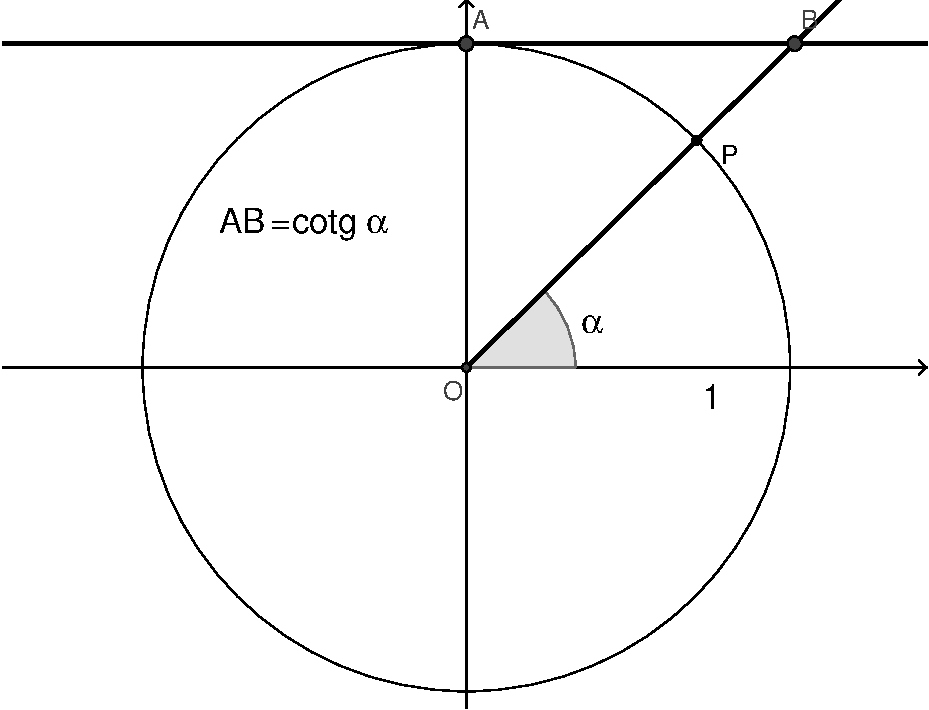
\includegraphics[scale=0.3]{cotgalpha-crop}
		\caption{Cotangente}\label{fig:CotangenteDefinizione}
	\end{subfigure}%
	\begin{subfigure}[b]{.5\linewidth}
		\centering\includegraphics[scale=0.3]{cotgalphagrafico-crop}
		\caption{Cotangente grafico}\label{fig:CotangenteGrafico}
	\end{subfigure}
	\captionof{figure}{Cotangente}
	\label{tab:funzcotg}
\end{figure}
\begin{definizione}[Cotangente]
	Data una circonferenza goniometrica\nobs\vref{fig:CotangenteDefinizione}, disegno un angolo con centro nell'origine e di ampiezza $\alpha$. Un lato dell'angolo incontra la tangente  alla circonferenza  per $(0;1)$ in un punto $C$.  Chiamo cotangente\index{Funzione!Cotangente!definizione} dell'angolo $\alpha$ e lo indico con $\cotg\alpha$ l'ascissa  del punto $C$
\end{definizione}
\subsection{Andamento Cotangente}
\label{sec:AndamentoCotangente}
\altapriorita{Inserire testo}
\begin{table}[tbp]
	\centering
	\renewcommand{\arraystretch}{2}
	\begin{tabular}{rccccc}
	\toprule
	%\backslashbox{Ottengo}{Noto} & $\sen\alpha$ &$\cos\alpha$&$\tg\alpha$ &$\cotg\alpha$ & \multirow{2}{1cm}{$\sen\alpha$ $\cos\alpha$} \\[.5cm]
	& $\sen\alpha$ &$\cos\alpha$&$\tg\alpha$ &$\cotg\alpha$ & $\sen\alpha$, $\cos\alpha$ \\[.6cm]
	\midrule
	$\cos\alpha={}$& $\pm\sqrt{1-\sen^2\alpha}$ & &$\pm\dfrac{1}{\sqrt{1+\tg^2\alpha}}$ & & \\ [.6cm]
	%\hline
	$\sen\alpha={}$& & $\pm\sqrt{1-\cos^2\alpha}$ &$\pm\dfrac{\tg\alpha}{\sqrt{1+\tg^2\alpha}}$ & & \\ [.6cm]
	%\hline
	$\tg\alpha={}$& & & & $\dfrac{1}{\cotg\alpha}$ &$\dfrac{\sen\alpha}{\cos\alpha}$\\ [.6cm]
	%\hline
	$\cotg\alpha={}$& & &$\dfrac{1}{\tg\alpha}$ & &$\dfrac{\cos\alpha}{\sen\alpha}$\\[.6cm] 
	\bottomrule
	\end{tabular}
	\caption{Seno Coseno Tangente Cotangente}
	\label{tab:SenoCosenoTangenteCotangente}
\end{table}
\renewcommand{\arraystretch}{1}
\section{Relazioni fondamentali}
\label{sec:RelazioniFondamentali}
\subsection{Seno e coseno}
\label{sec:RelazioniFondamentaliSenoCoseno}
\begin{definizione}[Relazione fondamentale goniometria]\index{Relazione!fondamentale goniometria}\index{Funzione!Seno}\index{Funzione!Coseno}
Dato un angolo $\alpha$ allora vale quanto segue:
\begin{equation}
\cos^2\alpha+\sen^2\alpha=1\label{eqn:RelazioneFondamentaleTrigonometria1}
\end{equation}
\end{definizione}
Dalla relazione\nobs\vref{eqn:RelazioneFondamentaleTrigonometria1} è possibile ottenere le seguenti
\begin{align}
&\cos^{2}\alpha={}1-\sen^{2}\alpha\\
&\cos\alpha={}\pm\sqrt{1-\sen^{2}\alpha}\\
&\sen^{2}\alpha={}1-\cos^{2}\alpha \\
&\sen^{2}\alpha={}\pm\sqrt{1-\cos^{2}\alpha}
\end{align}
Nella sezione\nobs\vref{sec:EsempiGoniometria} vi sono esempi per l'uso di queste formule
\subsection{Tangente cotangente}
\label{sec:TangenteCotangente}
\begin{definizione}[Tangente Cotangente]
	\index{Funzione!Tangente}\index{Funzione!Cotangente}\index{Funzione!Seno}\index{Funzione!Coseno}
	Dato un angolo $\alpha$ allora vale quanto segue:
\begin{align}
\tg\alpha=&{}\dfrac{\sen\alpha}{\cos\alpha}&\alpha&{}\neq\dfrac{\pi}{2}+k\pi\label{equ:tangente1}\\
\cotg\alpha=&{}\dfrac{\cos\alpha}{\sen\alpha}={}\dfrac{1}{\tg\alpha}& \alpha&{}\neq\pi\label{equ:cotangente1}
\end{align}
\end{definizione}
Dalle formule\nobs\vrefrange{equ:tangente1}{equ:cotangente1} è possibile ottenere le seguenti relazioni
\begin{align}
\cos^{2}\alpha=&{}\dfrac{1}{1+{\tg}^{2}\alpha} &\alpha&{}\neq\dfrac{\pi}{2}+k\pi\\
\cos\alpha=&{}\pm\dfrac{1}{\sqrt{1+{\tg}^{2}\alpha}} &\alpha{}&\neq\dfrac{\pi}{2}+k\pi\\
\sen^{2}\alpha=&{}\dfrac{\tg^{2}\alpha}{1+\tg^{2}\alpha}&\alpha{}&\neq\dfrac{\pi}{2}+k\pi\\
\sen\alpha=&{}\pm\dfrac{\tg\alpha}{\sqrt{1+\tg^{2}\alpha}}&\alpha{}&\neq\dfrac{\pi}{2}+k\pi
\end{align}
\section{Angoli associati}
\label{sec:goniometriaAngoliAssociati}
\subsection{Angoli supplementari}
Sono angoli la cui somma è $\ang{180}$, $\alpha$, $\ang{180}-\alpha$ la figura corrispondente è la\nobs\vref{fig:AngoliAssociatisupplementari}
\begin{figure}[H]
	\centering
\includestandalone[width=8.5cm]{funzgonioTikz/angoliassociati1}
	\caption{Angoli supplementari $\alpha$ $\ang{180}-\alpha$}
	\label{fig:AngoliAssociatisupplementari}
\end{figure}
Per questi angoli valgono le seguenti relazioni
\begin{align}
\cos\alpha=&{}-\cos(\ang{180}-\alpha)\\
\sen\alpha=&{}\sen(\ang{180}-\alpha)\\
\tg\alpha=&{}-\tg(\ang{180}-\alpha)\\
\cotg\alpha=&{}-\cotg(\ang{180}-\alpha)
\end{align}
\subsection{Angoli che differiscono di $\ang{180}$}
Sono angoli la cui differenza è $\ang{180}$, $\alpha$, $\ang{180}+\alpha$ la figura corrispondente è la\nobs\vref{fig:AngoliAssociatidiff180}
\begin{figure}[H]
	\centering
	\includestandalone[width=8.5cm]{funzgonioTikz/angoliassociati2}
			\caption{Angoli che differiscono di $\ang{180}$ $\alpha$ e $\ang{180}+\alpha$}
			\label{fig:AngoliAssociatidiff180}
\end{figure}
Per questi angoli valgono le seguenti relazioni
\begin{align}
\cos\alpha=&{}-\cos(\ang{180}+\alpha)\\
\sen\alpha=&{}-\sen(\ang{180}+\alpha)\\
\tg\alpha=&{}\tg(\ang{180}+\alpha)\\
\cotg\alpha=&{}\cotg(\ang{180}+\alpha)
\end{align}
\subsection{Angoli esplementari}
Sono angoli la cui somma è $\ang{360}$, $\alpha$, $\ang{360}-\alpha$ la figura corrispondente è la\nobs\vref{fig:Angolidif360}
\begin{figure}[H]
		\centering
			\includestandalone[width=7.0cm]{funzgonioTikz/angoliassociati3}
			\caption{Angoli esplementari $\alpha$ e $\ang{360}-\alpha$}
			\label{fig:Angolidif360}
	\end{figure}
Per questi angoli valgono le seguenti relazioni
\begin{align}
\cos\alpha=&{}\cos(\ang{360}-\alpha)\\
\sen\alpha=&{}-\sen(\ang{360}-\alpha)\\
\tg\alpha=&{}-\tg(\ang{360}-\alpha)\\
\cotg\alpha=&{}-\cotg(\ang{360}-\alpha)
\end{align}
\subsection{Angoli opposti}
Sono angoli la cui somma è $\ang{0}$, $\alpha$, $-\alpha$ la figura corrispondente è la\nobs\vref{fig:angoliopposti}
\begin{figure}[H]
	\centering
	\includestandalone[width=8.5cm]{funzgonioTikz/angoliopposti}
	\caption{Angoli opposti}
	\label{fig:angoliopposti}
\end{figure}
Per questi angoli valgono le seguenti relazioni
\begin{align}
\cos\alpha=&{}-\cos(-\alpha)\\
\sen\alpha=&{}-\sen(-\alpha)\\
\tg\alpha=&{}\tg(-\alpha)\\
\cotg\alpha=&{}\cotg(-\alpha)\\
\end{align}
\subsection{Angoli complementari}
Sono angoli la cui somma è $\ang{90}$, $\alpha$ e $\ang{90}-\alpha$ la figura corrispondente è la\nobs\vref{fig:angolicomplementari1}
\begin{figure}[H]
	\centering
	\includestandalone[width=8.5cm]{funzgonioTikz/angolicomplementari1}
		\caption{Angoli complementari $\alpha$ e  $\ang{90}-\alpha$}
		\label{fig:angolicomplementari1}
\end{figure}
Per questi angoli valgono le seguenti relazioni
\begin{align}
\cos\alpha=&{}\sen(\ang{90}-\alpha)\\
\sen\alpha=&{}\cos(\ang{90}-\alpha)\\
\tg\alpha=&{}\cotg(\ang{90}-\alpha)\\
\cotg\alpha=&{}\tg(\ang{90}-\alpha)
\end{align}
\subsection{Angoli che differiscono di $\ang{90}$}
Sono angoli la cui differenza è $\ang{90}$, $\alpha$ e $\ang{90}+\alpha$ la figura corrispondente è la\nobs\vref{fig:angolicomplementari2}
\begin{figure}[H]
	\centering
	\includestandalone[width=8.5cm]{funzgonioTikz/angolicomplementari2}
\caption{Angoli che differiscono di $\ang{90}$, $\alpha$ e $\ang{90}+\alpha$}
\label{fig:angolicomplementari2}
\end{figure}
Per questi angoli valgono le seguenti relazioni
\begin{align}
\cos\alpha=&{}\sen(\ang{90}+\alpha)\\
\sen\alpha=&{}-\cos(\ang{90}+\alpha)\\
\tg\alpha=&{}-\cotg(\ang{90}+\alpha)\\
\cotg\alpha=&{}-\tg(\ang{90}+\alpha)
\end{align}
\subsection{Angoli la cui somma è $\ang{270}$}
Sono angoli la cui somma è $\ang{270}$, $\alpha$ e $\ang{270}-\alpha$ la figura corrispondente è la\nobs\vref{tab:angolicomplementari3}
\begin{figure}[H]
	\centering
		\includestandalone[width=8.5cm]{funzgonioTikz/angolicomplementari3}
		\caption{Angoli la cui somma è $\ang{270}$,  $\alpha$ e $\ang{270}-\alpha$}
		\label{tab:angolicomplementari3}
\end{figure}
Per questi angoli valgono le seguenti relazioni
\begin{align}
\cos\alpha=&{}-\sen(\ang{270}-\alpha)\\
\sen\alpha=&{}-\cos(\ang{270}-\alpha)\\
\tg\alpha=&{}\cotg(\ang{270}-\alpha)\\
\cotg\alpha=&{}\tg(\ang{270}-\alpha)
\end{align}
\subsection{Angoli la cui somma è $\ang{270}$}
Sono angoli la cui differenza è $\ang{270}$, $\alpha$ e $\ang{270}+\alpha$ la figura corrispondente è la\nobs\vref{tab:angolicomplementari4}
\begin{figure}[H]
	\centering
		\includestandalone[width=8.5cm]{funzgonioTikz/angolicomplementari4}
		\caption{Angoli la cui differenza è $\ang{270}$, $\alpha$ e $\ang{270}+\alpha$}
		\label{tab:angolicomplementari4}
\end{figure}
Per questi angoli valgono le seguenti relazioni
\begin{align}
\cos\alpha=&{}-\sen(\ang{270}+\alpha)\\
\sen\alpha=&{}\cos(\ang{270}+\alpha)\\
\tg\alpha=&{}-\cotg(\ang{270}+\alpha)\\
\cotg\alpha=&{}-\tg(\ang{270}+\alpha)
\end{align}
%\mediapriorita{Manca la tabella 270+$\alpha$}
\begin{table}

	\centering
	\footnotesize
	\begin{tabular}{rlllllll}
	\toprule
	$\sen\alpha=$&$\cos(\ang{90}-\alpha)$&$-\cos(\ang{90}+\alpha)$&$\sen(\ang{180}-\alpha)$&$-\sen(\ang{180}+\alpha)$&$-\cos(\ang{270}-\alpha)$&$\cos(\ang{270}+\alpha)$&$-\sen(-\alpha)$\\[.6cm] 
	$\cos\alpha=$&$\sen(\ang{90}-\alpha)$&$\sen(\ang{90}+\alpha)$&$-\cos(\ang{180}-\alpha)$&$-\cos(\ang{180}+\alpha)$&$-\sen(\ang{270}-\alpha)$&$-\sen(\ang{270}+\alpha)$&$\cos(-\alpha)$\\[.6cm] 
	$\tg\alpha=$&$\cotg(\ang{90}-\alpha)$&$-\cotg(\ang{90}+\alpha)$&$-\tg(\ang{180}-\alpha)$&$\tg(\ang{180}+\alpha)$&$\cotg(\ang{270}-\alpha)$&$-\cotg(\ang{270}+\alpha)$&$-\tg(-\alpha)$\\[.6cm] 
	$\cotg\alpha=$&$\tg(\ang{90}-\alpha)$&$-\tg(\ang{90}+\alpha)$&$-\cotg(\ang{180}-\alpha)$&$\cotg(\ang{180}+\alpha)$&$\tg(\ang{270}-\alpha)$&$-\tg(\ang{270}+\alpha)$&$-\cotg(-\alpha)$\\[.6cm]
	\bottomrule
	\end{tabular}
	\caption{Angoli complementari e supplementari}
	\label{tab:differnzediangoli}
\end{table}
La tabella\nobs\vref{tab:differnzediangoli} riassume i risultati precedenti.
%\section{Formule di addizione e sottrazione}
%\label{sec:Formulediaddizionesottrazione}
%\altapriorita{Inserire testo}
%\subsection{Coseno della differenza di due angoli}
%\label{sec:cosenodifferenza}
%\begin{figure}
%	\centering
%\includestandalone[width=8.5cm]{funzgonioTikz/cosenosommadifferenza1}
%	\caption{Differenza di angoli}
%	\label{fig:DifferenzaCosenoAngoli}
%\end{figure}
%\begin{table}
%	\centering
%	$
%	\begin{array}{cc}
%	\toprule
%	\cos(\alpha-\beta)=	&\cos\alpha\cos\beta+\sen\alpha\sen\beta \\ 
%	\cos(\alpha+\beta)=	&\cos\alpha\cos\beta-\sen\alpha\sen\beta \\ 
%	\sen\left(\alpha-\beta\right)={} &\sen\alpha\cos\beta-\cos\alpha\sen\beta\\
%\sen\left(\alpha+\beta\right)={}&\sen\alpha\cos\beta+\cos\alpha\sen\beta\\
%	\bottomrule
%	\end{array}
%	$ 
%	\caption{Seno e Coseno, somma o differenza di angoli}
%	\label{Tab:sommadifferenzacosenoseno}
%\end{table}
\section{Equazioni goniometriche elementari}
\label{sec:EquazioniGoniometricheElementari}
Le funzioni goniometriche elementari sono equazioni del tipo
\begin{align*}
	\sen x&=m&\cos x&=n&\tg x&=q
\end{align*}
\subsection{$\sen x=m$}
Il seno di un angolo è una funzione limitata con valori compresi tra meno uno ed uno $(1\leq\sen x\leq 1)$ quindi l'equazione è impossibile per valori di $m$ esterni a tale intervallo. Abbimo vari casi:
\begin{description}
	\item[$0<m<1$] In questo caso le soluzioni sono due come nella figura\nobs\vref{fig:senelemen1} $x=\alpha+k\ang{360}$ e $x=\ang{180}-\alpha+k\ang{360}$
\end{description} 

\begin{figure}
	\centering
		\begin{tikzpicture}[>=triangle 45]
		% draw the coordinates
		\pgfmathsetmacro{\raggio}{4};
		\pgfmathsetmacro{\pangolo}{20};
		\pgfmathsetmacro{\sangolo}{{180-\pangolo}};
		\pgfmathsetmacro{\mraggio}{\raggio/3};
		\pgfmathsetmacro{\sraggio}{1.9*\raggio};
		% draw the unit circle
		\draw[->] (0,-\raggio-\mraggio) -- (0,\raggio+\mraggio) node[above,fill=white] {$y$};
		\draw[->] (-\raggio-\mraggio,0) -- (\raggio+\mraggio,0) node[right,fill=white] {$x$};
		\draw[thick] (0,0) circle(\raggio);
		\coordinate [label= below left:$O$] (OO)at(0,0);
		\coordinate (P)  at ({\raggio*cos(\pangolo},{\raggio*sin(\pangolo});
		\coordinate (Pr)  at ({\mraggio+\raggio*cos(\pangolo},{\raggio*sin(\pangolo});
		\coordinate (PX)  at ({\raggio*cos(\pangolo},0);
		\coordinate (PY)  at (0,{\raggio*sin(\pangolo});
		\coordinate (Q)  at ({\raggio*cos(\sangolo},{\raggio*sin(\sangolo});
		\coordinate (Qr)  at ({-\mraggio+\raggio*cos(\sangolo},{\raggio*sin(\sangolo});
		\coordinate (QX)  at ({\raggio*cos(\sangolo},0);
		\coordinate (QY)  at (0,{\raggio*sin(\sangolo});
		\coordinate (M)  at (0,{\raggio*sin(\sangolo});
		\node at (P) [label=above right:$m$]{};
		%\node at (Q) [label=left:$Q$]{};
		\fill [color=black] (OO) circle (1.5pt);
		\fill [color=black] (P) circle (1.5pt);
		%\fill [color=black] (PX) circle (1.5pt);
		%\fill [color=black] (PY) circle (1.5pt);
		%\fill [color=black] (M) circle (1.5pt);
		\fill [color=black] (Q) circle (1.5pt);
		%\fill [color=black] (QX) circle (1.5pt);
		%\fill [color=black] (QY) circle (1.5pt);
		%\draw[->] {(\sraggio/2.5},0 ) arc (0:\pangolo:\sraggio/2.5) node[above] {$\arco$};
		\draw(Pr)--(Qr);
		\draw(P)--(PY);% node[midway,above] {$ cos(\alpha)$};
		\draw(Q)--(QY);% node[midway,above] {$cos(ang{180}-\alpha)$};
		%\draw(P)--(PX);% node[midway,above,right] {$sen(\alpha)$};
		%\draw(Q)--(QX);%node[midway,below,left] {$sen(ang{180}-\alpha)$};
		\draw [->] (0:\sraggio/3) arc (0:\sangolo:\sraggio/3) node[sloped,below right] {$\ang{180}-\alpha$};
		\draw [->] (0:\sraggio/4) arc (0:\pangolo:\sraggio/4) node[above] {$\alpha$};
		\draw(OO)--(P);
		\draw(OO)--(Q);
		\end{tikzpicture} 
	\captionof{figure}{$\sen x=m$ $0<m<1$}
	\label{fig:senelemen1}
\end{figure}